
\section{Evaluation}\label{sec:evaluation}

In evaluating the real-time efficacy of the Raspberry Pi 3, the same methodology is utilized in all 
experiments conducted. The performance of the Pi is measured over a set of 1001 video frames that are 
each individually fed to the model. The processing time for the first frame is ignored as, due to 
cache warmup, it is uncharacteristically high and doesn't accurately represent the Pi's capabilities. A 
deadline of 50 ms, or 20 Hz, is used as a baseline to assess the Pi's ability to complete all 
necessary real-time operations in a timely manner. Also, please note that frame processing times 
would be approximately the same if the input stream was a 
camera instead of a video. 

\subsection{Real-Time Operations}
In a real-time operations, the system has to be capable of consistently executing all necessary 
functions before their given deadlines. In the case of our platform, it has to process every given frame 
and get the predicted angles from the model. In order to determine if the Raspberry Pi 3 is capable of 
this, we tested the platform and recorded the time it took for the Pi to complete all real-time 
functions for every given frame.For this experiment, all four of the Pi's cpu cores were utilized, and 
only one model was run. As can be seen in Figure 1, the Pi was able to meet almost all of its deadlines, 
while only missing it in a few instances.

\begin{figure}[h]
  \centering
  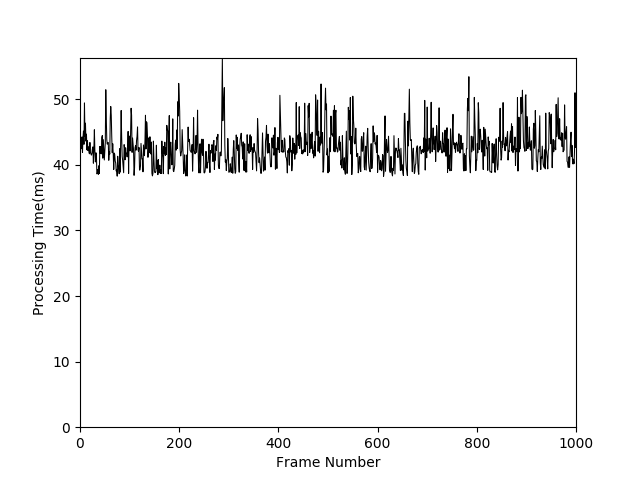
\includegraphics[width=.5\textwidth]{Total_Processing_Time}
  \caption{ Real-time performance of the Raspberry Pi 3 in processing 1000 frames.}
\end{figure}

In our platform, three main real-time tasks are performed during autonomous operation. 
In order, those operations are: (1) capturing and reading the input frame from the designated camera 
or video stream, (2) preprocessing the acquired frame so that it is compatible with the DNN, and (3) 
feeding the frame to, and getting the angle prediction from, the model. However, the time it takes to 
complete each of the operations will differ, with at least one of them being the dominating step in 
processing each frame.

\begin{table}[h]
  \centering
  \begin{tabular} {| l | l | l | l | l |}
    \hline
    \textbf{operation} & \textbf{mean} & \textbf{max} & \textbf{99pct} & \textbf{stdev} \\ \hline 
    Frame Capture & 2.28 & 4.94 & 63.31 &  .51\\ \hline
    Preprocessing & 3.09 & 4.6 & 3.31 & .1 \\ \hline
    Angle Prediction & 37.3 & 51.03 & 45.48 & 2.75 \\ 
    \hline
  \end{tabular}
  \caption{Real-time performance of the Raspberry Pi 3 depending on the number of cores used.}
\end{table}

In order to determine which operation(s) take the longest to execute, we measured the time it 
took for each step to be completed. For this experiment, all four of the Pi's cpu cores were utilized, 
and only one model was run. As is shown in Fig. 1, the angle prediction operation (3) consumes the 
majority of the processing for each frame. Furthermore, the time it takes for the operation to 
complete is volatile, and can range anywhere between 30 ms and 50 ms for any particular frame. On the 
other hand, both the frame capture (1) and preprocessing (2) operations take substantially less time 
and are relatively more consistent in their times, at 2 ms and 3 ms, respectively. 

\subsection{Multicore Performance}
It may not always be the case that all four cores of the Raspberry Pi 3's Cortex A-53 CPU can be used 
solely for the purpose of operating an autonomous vehicle. Thus, we test how the number of cores 
utilized for real-time operations affects the Pi's overall ability to function as an autonomous 
vehicle platform.

\begin{table}[h]
  \centering
  \begin{tabular} {| l | l | l | l | l | l | l | l | l | l |}
    \hline
    \textbf{num cores} & \textbf{mean} & \textbf{max} & \textbf{99pct} & \textbf{stdev} \\ \hline 
    1 & 61.96 & 66 & 63.31 &  .51\\ \hline
    2 & 50.49 & 71.55 & 70.03 & 4.18 \\ \hline
    3 & 48.11 & 72.22 & 58.45 & 2.8 \\ \hline
    4 & 42.67 & 56.37 & 50.70 & 2.8 \\
    \hline
  \end{tabular}
  \caption{Real-time performance of the Raspberry Pi 3 depending on the number of cores used.}
\end{table}

As is depicted in Table 1, the Raspberry Pi performed better, on average, when it utilized more 
cores. With 4 cores, the Pi was able to meet the vast majority of its 50 ms deadlines, doing so in 
almost 99\% of the processed frames. The Pi had the worst average performance when using only 1 core, 
as it was unable to meet any of the 50 ms deadlines (its fastest processing time was just under 60 
ms). Another observation is that the difference between using 2 cores and 3 cores is relatively 
small. On average, using 3 cores only performed better by 2 ms, so the addition of one core in that 
specific case offers relatively little improvement. However, please note that the average time when 
using 3 cores was below the 50 ms deadline, while the average time using 2 cores was slightly above it. 
One important observation that can be made is that of consistency, as using only 1 core had a much 
steadier performance. As a result, the use of multiple cores is very beneficial in terms of reducing 
the time it takes to complete real-time operations, but may ultimately result in processing times 
that are more volatile.

\subsection{Multimodel Performance}
In a real world scenario, it is highly probable that multiple models will need to be used 
simultaneously in order to perform various important tasks (angle prediction, object detection, 
etc.)\cite{}. As such, we also tested the capability of the Raspberry Pi to run multple models at the 
same time, and measure whether all models are able to meet their respective deadlines on a consistent 
basis. Specifically, the Pi is tested in the cases of running 2 and 4 models simultaneously. For each 
case, all models are allocated an equal number of cores, with 2 models having 2 cores each, and 4 
models having 1 core each.

\begin{table*}
  \begin{tabular} {| l | l | l | l | l | l | l | l | l |}
  \hline
  \textbf{num models} & \textbf{cores} & \textbf{mean} & \textbf{L1 refs} & \textbf{L1 
    misses} & \textbf{L1 miss \%} & textbf{L2 refs} & \textbf{L2 misses} & \textbf{L2 miss \%} \\ \hline
  1 & 0,1 & 51.35 & 3.04E+10 & 4.78E+08 & 1.58 & 3.31E+09 & 3.68E+08 & 11.12\\ \hline
  2 & 0,1 & 58.03 & 3.04E+10 & 4.91E+08 & 1.61 & 3.91E+09 & 4.26E+08 & 10.88 \\ \hline
  2 & 2,3 & 56.4 & 3.04E+10 & 4.80E+08 & 1.58 & 3.88E+09 & 4.21E+08 & 10.87 \\ \hline
  \end{tabular}
  \caption{Real-time performance of the Raspberry Pi 3 when 2 models are running simultaneously.}
\end{table*}

Ideally, each model run would replicate a single model run. However, Table 2 shows that such was not 
the case. In the tests where 2 models ran simultaneously, both of the models showed average time 
increases of around 5-7 ms, around 10\%, when compared to a baseline of 1 model running on two cores. 
This change, however, did not seem to be caused by any form of cache interference as both L1 and L2 
cache misses remained constant, regardless of the number of models running. The number of L1 misses 
being close to 1.6\% of all references and the number of L2 misses being about 11\% of all 
references.

\begin{table*}
  \begin{tabular} {| l | l | l | l | l | l | l | l | l |}
  \hline
  \textbf{num models} & \textbf{core} & \textbf{mean} & \textbf{L1 refs} & \textbf{L1 
    misses} & \textbf{L1 miss \%} & textbf{L2 refs} & \textbf{L2 misses} & \textbf{L2 miss \%} \\ \hline
    1 & 0 &  62.48 & 2.78E+10 & 4.36E+08 & 1.57 & 2.83E+09 & 3.59E+08 & 12.68  \\ \hline
    4 & 0 & 77.9 & 2.79E+10 & 4.53E+08 & 1.63 & 3.36E+09 & 4.43E+08 & 13.19 \\ \hline
    4 & 1 & 78.89 & 2.79E+10 & 4.64E+08 & 1.67 & 3.42E+09 & 4.38E+08 & 12.82 \\ \hline
    4 & 2 & 77.81 & 2.78E+10 & 4.45E+08 & 1.6 & 3.45E+09 & 4.41E+08 & 12.77 \\ \hline
    4 & 3 & 77.87 & 2.79E+10 & 4.45E+08 & 1.60 & 3.41E+09 & 4.39E+08 & 12.88 \\ \hline
  \end{tabular}
  \caption{Real-time performance of the Raspberry Pi when 4 models are running simultaneously.}
\end{table*}

The difference was even greater in the case of 4 models running concurrently, as each one displayed 
an average time increase of approximately 15 ms, around 30\%, when compared to a single model 
running on 1 core. Once again, though, cache interference was not a factor as the number of L1 cache 
misses remained 1.6\% of all references, and the number of L2 cache misses stayed at 13\% of all 
references.

\subsection{Performance Requirements}
In the utilization of the Raspberry Pi 3 in our platform, there are a few factors that need to be 
considered and/or enforced in order to guarantee that the Pi is able to consistently perform at a 
desired level. Specifically, these issues all have the potential to negatively affect the cpu clock 
speed/frequency, which would result in decreased performance. While, in the above experiments, the cpu 
operated at a preferred clock speed of 1.2 GHz, it is entirely possible for the cpu to operate at a 
lower frequency if the following problems are not taken into account.

The most notable issue that can affect the cpu clock speed is that of the power supplied to the 
Raspberry Pi. In essence, it is necessary that the Pi be supplied with 2 Amps, as any less could 
hinder the Pi's ability to maintain a 1.2 GHz frequency. In experiments done with a power supply that 
only provided 1 Amp, the Pi was unable to sustain a 1.2 GHz clock speed and, instead, fluctuated 
between operating at 600 MHz and 1.2 GHz. As a result, it is necessary, or at least highly 
recommended, that the power supply used for the Raspberry Pi 3 be capable of outputting 2 Amps, 
otherwise optimal performance isn't guaranteed.

Another factor that can affect clock speed is that of the cpu's temperature. Some model operations can 
be computationally intensive, thus it is possible for the temperature of the cpu to become relatively 
high. This can be especially problematic in situations where multiple models are running 
simultaneously on the Pi. As a consequence, thermal throttling may be used to decrease the clock 
speed so that the cpu temperature stays at a safe level. As such, the Raspberry Pi may not be suited 
for prolonged use, especially in cases where the workload is relatively larger, like running multiple 
models. Rather, the Pi seems to be better suited for running in set periods, after which it is turned 
off or made idle so that the cpu is given time to cool down.
